\documentclass[12pt]{article}
\usepackage{graphicx}
\usepackage{enumerate}
\usepackage{amsmath}
\usepackage{amssymb}
\usepackage[mathscr]{euscript}
\usepackage{hyperref}
\usepackage{bbm}

\hypersetup{
    colorlinks=true,
    urlcolor=blue
}

\setlength{\oddsidemargin}{.1in}
\setlength{\textwidth}{6.3in}
\setlength{\textheight}{8.9in}
\setlength{\topmargin}{-.5in}

\title{Solving the inverted pendulum as a Markov decision problem}
\date{}

\begin{document}

\maketitle

\section{Markov decision problems}

A Markov decision problem (MDP) is defined by a 5-tuple $(\mathscr{S}, \mathscr{A}, P_\cdot(\cdot, \cdot), R_\cdot(\cdot, \cdot), \gamma)$ where

\begin{enumerate}[(i)]
\item $\mathscr{S}$ is a finite set of states;
\item $\mathscr{A}$ is a finite set of actions;
\item $P_a(s, s')$ is the probability that action $a$ in state $s$ at time $t$ will lead to state $s'$ at time $t + 1$;
\item $R_a(s, s')$ is the immediate reward received after transitioning from state $s$ to state $s'$ due to action $a$; and
\item $\gamma \in [0, 1]$ is a discount factor which represents the difference in importance between future rewards and present rewards.
\end{enumerate}

The problem is to find a policy for a decision-making agent that navigates the states of this world via actions. The policy is a function $\pi$ that specifies the action $\pi(s)$ that the agent will choose when in state $s$. Our goal is to choose a policy that will maximize a cumulative function of the random rewards; in particular, we wish to maximize the discounted sum of expected rewards over a potentially infinite horizon:

\begin{equation}
\sum_{t = 0}^{\infty} \gamma^t \mathbb{E}[R_{a_t}(s_t, s_{t+1})] \quad \mbox{where } a_t = \pi(s_t).
\end{equation}

\subsection{Policies and value functions}

Imagine that we have some magical function $V(\cdot)$ which tells us the inherent value of a state. It accepts a state as its argument, and its output value tells us \emph{how characteristically good} it is to be in that state for the purposes of achieving our goal (that is, maximizing reward). A bit philosophical, eh?

If we had this function, then choosing a policy would be trivial: the optimal policy is one which always selects the action that maximizes the expectation of $V(s')$ based on the present state $s$. The expectation of $V(s')$ under a given action $a$ in state $s$ is a sum of $V(s')$ over all possible $s'$, with each term weighted by the probability of transitioning from $s$ to $s'$ due to action $a$:

\begin{equation}
\mathbb{E}[V(s')] = \sum_{s' \in \mathscr{S}} P_a(s, s') V(s').
\end{equation}

So the optimal policy is

\begin{equation}
\pi^*(s) = \underset{a}{\arg\max} \, \mathbb{E}[V(s')] = \underset{a}{\arg\max} \, \sum_{s' \in \mathscr{S}} P_a(s, s') V(s').
\end{equation}

But, the inherent value of a state $V(\cdot)$ depends on what policy we are following. In particular, it is the sum of the expected reward over all future times if we act according to a policy $\pi$. Intuitively, there are two factors which influence the value of state $s$:

\begin{enumerate}[(i)]
\item{the immediate expected reward of acting on our policy in state $s$} and
\item{the expected value of the state which follows from acting on our policy in state $s$.}
\end{enumerate}

Note that the second of these is defined in terms of the expected value of the state which follows. Thus, our description of the value of state $s$ includes the value of state $s'$, and in this way recursively depends on the value of all future states which will follow.

Let's work out each of the two factors above, starting with the first piece. The expected reward of taking action $a$ in a given state $s$ is a sum of $R_a(s, s')$ over all possible $s'$, with each term weighted by the probability of transitioning from $s$ to $s'$ due to action $a$:

\begin{equation}
\mathbb{E}[R_a(s)] = \sum_{s' \in \mathscr{S}} P_a(s, s') R_a(s, s').
\end{equation}

The action $a$ is selected by policy $\pi(s)$, so we can rewrite our equation above as the expected reward of acting under policy $\pi$ in a given state $s$:

\begin{equation}
\label{eq:reward} \mathbb{E}[R_{\pi(s)}(s)] = \sum_{s' \in \mathscr{S}} P_{\pi(s)}(s, s') R_{\pi(s)}(s, s').
\end{equation}

This is our expression for the immediate expected reward of acting on our policy in state $s$ (the first of the two factors mentioned above). But the value of state $s$ depends not only on this immediately available reward; it also depends on the expected value of the state which follows from acting on our policy (the second of the two factors above):

\begin{equation}
\label{eq:future_value} \mathbb{E}[V(s')] = \sum_{s' \in \mathscr{S}} P_{\pi(s)}(s, s') V(s').
\end{equation}

The full value of state $s$ is a sum of equations (\ref{eq:reward}) and (\ref{eq:future_value}), with the second weighted by our discount factor to reflect the fact that this is the value of a state ($s'$) which is one step ahead in the future from the state ($s$) whose value we are presently considering. So, to get the value of state $s$ under policy $\pi$, we sum the expectation of the immediate reward for acting on our policy from state $s$ and the future-discounted expectation of the value of the state $s'$ which follows from acting on our policy in state $s$:

\begin{align}
V(s) &= \mathbb{E}[R_{\pi(s)}(s)] + \gamma \mathbb{E}[V(s')] \\[5pt]
&= \sum_{s' \in \mathscr{S}} P_{\pi(s)}(s, s') R_{\pi(s)}(s, s') + \gamma \sum_{s' \in \mathscr{S}} P_{\pi(s)}(s, s') V(s') \\[5pt]
&= \sum_{s' \in \mathscr{S}} P_{\pi(s)}(s, s') \Big(R_{\pi(s)}(s, s') + \gamma V(s')\Big)
\end{align}

Let's take stock. We have an expression for the optimal policy with respect to any given value function, and we have an expression for a value function under a given policy. To reiterate:

\begin{align}
\pi^*(s) &= \underset{a}{\arg\max} \, \mathbb{E}[V(s')] = \underset{a}{\arg\max} \, \sum_{s' \in \mathscr{S}} P_a(s, s') V(s') \\[5pt]
V(s) &= \sum_{s' \in \mathscr{S}} P_{\pi(s)}(s, s') \Big(R_{\pi(s)}(s, s') + \gamma V(s')\Big)
\end{align}

\subsection{The Bellman optimality equations}

But now we have a bit of a conundrum. We know the optimal policy with a given a value function, but our value function itself depends on what policy we're acting under! How do we find, at once, the optimal value function and its optimal policy?

For any given state, there exists a large space of possible value functions due to all possible policies we could use. Consider for a moment that we are handed, from on high, the optimal policy for our task. Under this policy, the output of the value function would be greater than or equal to the output of the value function under any other policy. This is because the optimal policy necessarily maximizes the value of any state. So, policies give an ordering over all value functions, and the maximal value function for a state coincides with acting under a perfect policy, or taking the best possible action for that state.

So, we can readily define a notion of the optimal value function. The optimal value function for a state must equal the value function for that state under the best possible action for that state:

\begin{equation}
V^*(s) = \underset{a}{\max} \, V(s).
\end{equation}

Note that in this case, the action $a$ is the optimal policy $\pi^*(s)$. This enables us to write out $V(s)$ with no reference to $\pi(s)$ at all, instead substituting $\pi(s) = a$:

\begin{equation}
V^*(s) = \underset{a}{\max} \, \sum_{s' \in \mathscr{S}} P_{\pi(s)}(s, s') \Big(R_{\pi(s)}(s, s') + \gamma V^*(s')\Big).
\end{equation}

This requires solving a set of $|\mathscr{S}|$ nonlinear recurrence relations in $|\mathscr{S}|$ variables\footnotemark, each one requiring a maximum over $|\mathscr{A}|$ expressions ($|\mathscr{A}|$ and $|\mathscr{S}|$ are the number of elements in the sets $\mathscr{A}$ and $\mathscr{S}$, respectively). These are called the \emph{Bellman equations} for an optimal value function. Intuitively, solving each one amounts to finding the value functions which result from trying each available action in a state, and then selecting the value function which corresponds to the best action in that state (the value function for that state under an optimal policy). Solving them all simultaneously amounts to finding the value function under an optimal policy for all states at once, yielding the full optimal value function.

\footnotetext{Such systems generally cannot be characterized analytically and lack a closed-form solution. In fact, solving nonlinear recurrence relations is often viewed as a hopeless endeavor: to solve \emph{every} nonlinear recurrence relation would imply that one could solve the Halting problem, as one could encode a program as initial states and the workings of the Turing machine as the recurrence relations (see \href{https://math.stackexchange.com/users/11513/rex-kerr}{this Stack Exchange discussion} by Rex Kerr). But these equations can be solved numerically (at least in principle), and with sufficiently small action and state spaces this computation is tractable. This where we're headed.}

Once we have $V^*(s)$, we can substitute this back into our expression for $\pi^*(s)$:

\begin{equation}
\pi^*(s) = \underset{a}{\arg\max} \, \sum_{s' \in \mathscr{S}} P_a(s, s') V^*(s').
\end{equation}

This is an optimal policy, and our solution to the MDP.

\section{The inverted pendulum problem as an MDP}

To set up the inverted pendulum problem as an MDP, we need to define for our agent

\begin{enumerate}[(i)]
\item{a world of available states,}
\item{a set of actions it can take,}
\item{the transition probabilities which describe the physical dynamics of this world,}
\item{a reward function which incentivizes remaining balanced upright, and}
\item{a discount factor which reflects how long- or short-sighted our agent is.}
\end{enumerate}

\subsection{The agent's world}

First we will build the world of our agent by choosing (i) and (ii): the states it can visit and the actions it can take. The computational complexity of solving the Bellman equations explodes rapidly as the combinations of possible states and actions grow. So, our choices of (i) and (ii) ultimately depend on how long we are willing to wait, and unfortunately it doesn't take much to have to wait an astronomically period time. Since we're not willing to wait the age of the universe, our state and action spaces will have to be pretty small indeed.

Let's begin with a state space for our agent. The state of the pendulum-cart system can be fully characterized by four variables: angular position of the pendulum, angular velocity of the pendulum, position of the cart, and velocity of the cart. In order to avoid our state space becoming overly large, we will have to discretize each of these continuous variables into distressingly course-grained substates.

First let's consider the pendulum. For the angular position subspace $\mathscr{S}^\theta$, we choose the four substates

\begin{equation}
s^\theta = \left\{
\begin{array}{lr}
s_1^\theta \quad : -\pi \leq \theta < -\frac{\pi}{2} \\
s_2^\theta \quad : -\frac{\pi}{2} \leq \theta < 0 \\
s_3^\theta \quad : 0 \leq \theta < \frac{\pi}{2} \\
s_4^\theta \quad : \frac{\pi}{2} \leq \theta < \pi
\end{array}
\right.
.
\end{equation}

\begin{figure}
\center
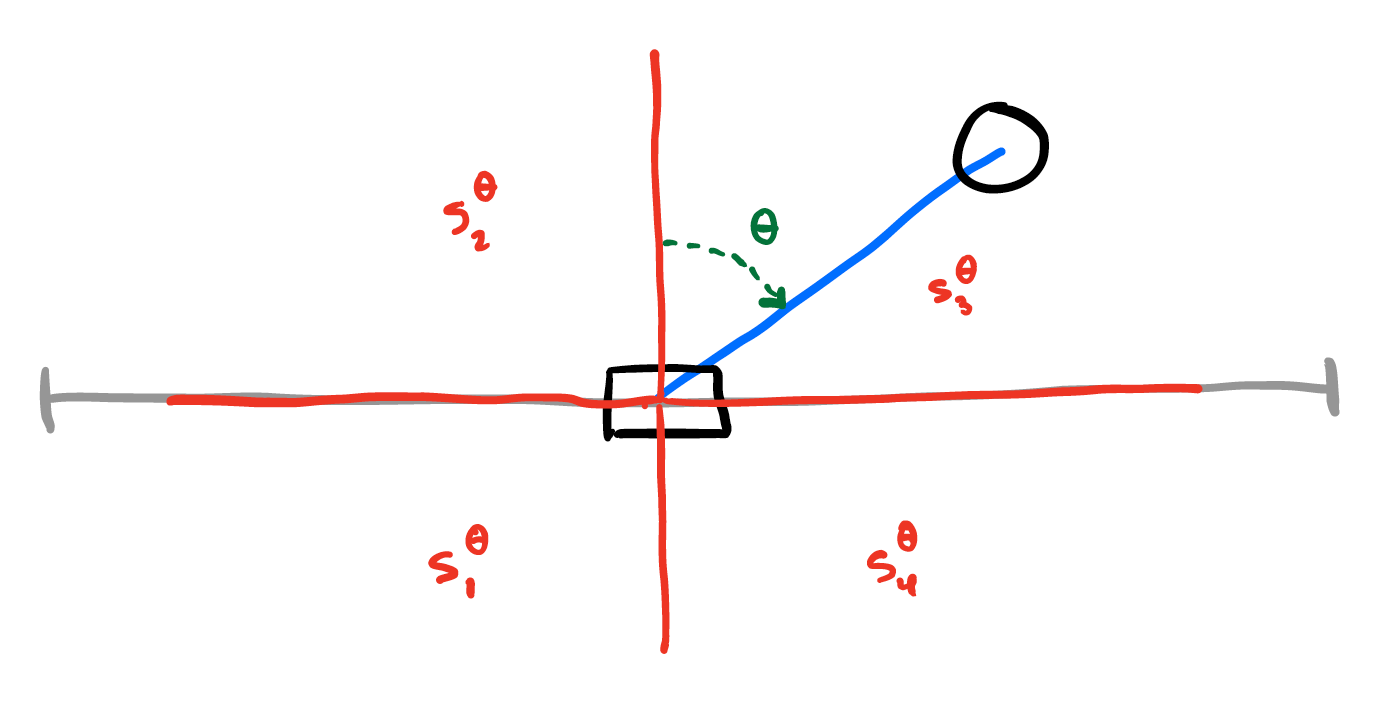
\includegraphics[width=0.9\linewidth]{substates.png}
\caption{Visualization of the substate space for angular position.}
\label{fig:substates}
\end{figure}

For the angular velocity subspace $\mathscr{S}^\omega$, we similarly choose four substates

\begin{equation}
s^\omega = \left\{
\begin{array}{lr}
s_1^\omega \quad : \omega < -\alpha \\
s_2^\omega \quad : -\alpha \leq \omega < 0 \\
s_3^\omega \quad : 0 \leq \omega < \alpha \\
s_4^\omega \quad : \alpha \leq \omega
\end{array}
\right.
\end{equation}

where $\alpha$ is a parameter deciding the `width' of our state bins.

Now on to the cart. For its position subspace $\mathscr{S}^x$, we choose the four substates

\begin{equation}
s^x = \left\{
\begin{array}{lr}
s_1^x \quad : x < -\beta \\
s_2^x \quad : -\beta \leq x < 0 \\
s_3^x \quad : 0 \leq x < \beta \\
s_4^x \quad : \beta \leq x
\end{array}
\right.
\end{equation}

and for its velocity subspace $\mathscr{S}^v$ we choose four substates

\begin{equation}
s^v = \left\{
\begin{array}{lr}
s_1^v \quad : v < -\eta \\
s_2^v \quad : -\eta \leq v < 0 \\
s_3^v \quad : 0 \leq v < \eta \\
s_4^v \quad : \eta \leq v
\end{array}
\right.
\end{equation}

where $\beta$ and $\eta$ are again parameters deciding the `width' of the state bins.

The full state space $\mathscr{S}$ is $\mathscr{S}^\theta \times \mathscr{S}^\omega \times \mathscr{S}^x \times \mathscr{S}^v$, or the set of all ordered pairs $(s^\theta, s^\omega, s^x, s^v)$. By our choices above, this space has 256 states.

Our agent acts by applying horizontal forces to the cart. We'll allow our agent to choose among five actions, each applying a different, discrete-valued force to the cart:

\begin{equation}
\mathscr{A} = \left\{a_1, a_2, a_3, a_4, a_5\right\} \mbox{ where }\left\{
\begin{array}{lr}
a_1 \quad : f = -\kappa_2 \\
a_2 \quad : f = -\kappa_1 \\
a_3 \quad : f = 0 \\
a_4 \quad : f = \kappa_1 \\
a_5 \quad : f = \kappa_2
\end{array}
\right.
.
\end{equation}

$\kappa_1$ and $\kappa_2$ are parameters deciding the force of the action.

\subsection{How the world works}

Now our agent needs a model of the physical dynamics of its world and how its actions affect those dynamics. This model comes in the form of a set of transition probabilities $P_a(s, s')$---one for every possible action $a$---describing the probability of transitioning from state $s$ to state $s'$ due to that action.

In our case the transition probabilities represent the physics of the pendulum-cart system. However, forming these transition probabilities is not totally straightforward: the states which describe our system each contain a wide, continuous range of actual physical configurations, leaving a great range of physical variability over which state will proceed from which. So, we will produce the transition probabilities via a Monte Carlo estimate of randomly simulated dynamics. For each state $a$ and state $s$, we'll randomly sample an angular position and velocity uniformly from within the state $s$, and run the simulation one step forward to end up in state $s_{next}$. We'll repeat this a large number of times $N$ and estimate the transition probabilities as

\begin{equation}
P_a(s, s') = \frac{1}{N}\sum_{i = 1}^N \mathbbm{1}(s_{next} = s').
\end{equation}

Since the most extreme states for velocity and angular velocity cover an unbounded range of physical possibilities (off to velocities of positive and negative $\infty$), we'll just have to choose physically realistic boundaries for the sake of sampling.

This is going to be an inherently flawed estimate. We're estimating the dynamics by sampling uniformly from the continuum of available positions and velocities within each state; yet in reality, there's no reason the physical system should visit all possible (continuous) positions and velocities within a state with equal probability. Nonetheless, let's consider this satisfactory, reasoning that our estimate of the transition probabilities should encode no finer-grained statistical assumptions about our system than our agent's representation of its state allows.\footnotemark

\footnotetext{Note that if we \emph{could} choose arbitrarily fine-grained states, this issue would go away: as the state ``slices" grew thinner, the physical dynamics of the system would become far less variable within each one, and our estimate of their transition probabilities would increasingly-well approximate the dynamics of the physical system. Furthermore, these transition probabilities would become increasingly sparse, reflecting the fact that in a causally deterministic system each state may transition to only one other state with unity probability. But alas, our agent must content itself to inhabit a simple---and unsettlingly noisy---world.}

\subsection{What the agent wants}

Next we need to construct a reward function that incentivizes our agent to do the right thing. Roughly, we would like our agent to balance the pendulum and remain near the center of the track. This means there are two things we wish to avoid:

\begin{enumerate}[(i)]
\item{allowing the pendulum to fall below the level of the track and}
\item{moving the cart too close to the ends of the track.}
\end{enumerate}

So, we will let the reward function equal -1 for any action taken in any state that satisfies either of these conditions, and 0 otherwise:

\begin{equation}
R_a(s, s') = \left\{
\begin{array}{lr}
-1 \quad : s^\theta \in \left\{s_1^\theta, s_4^\theta \right\}\mbox{ or }s^x \in \left\{s_1^x, s_4^x \right\} \\
0 \quad : \mbox{otherwise}
\end{array}
\right.
.
\end{equation}

Finally, we make sure to choose a discount factor $\gamma$ as well. Having fleshed out $\mathscr{S}$, $\mathscr{A}$, $P_\cdot(\cdot, \cdot)$, $R_\cdot(\cdot, \cdot)$, and $\gamma$, we have fully set up our inverted pendulum problem as an MDP. The rest is up to the Bellman equations.

\end{document}